% Chapter 1
\stepcounter{cap}
%\chapter{cap1}
\label{cap4}

\mychapter{4}{Capitolul \arabic{cap} \\ STRUCTURA BAZEI DE DATE}
%\chapter{\arabic{cap}.Introducere} % Main chapter title

\label{Chapter4} % For referencing the chapter elsewhere, use \ref{Chapter1} 

\thispagestyle{fancy}

%-----------------------------------------------------------------
\section{Tabelele de date}


\begin{figure}[h!]
  \centering
    \centering{%
      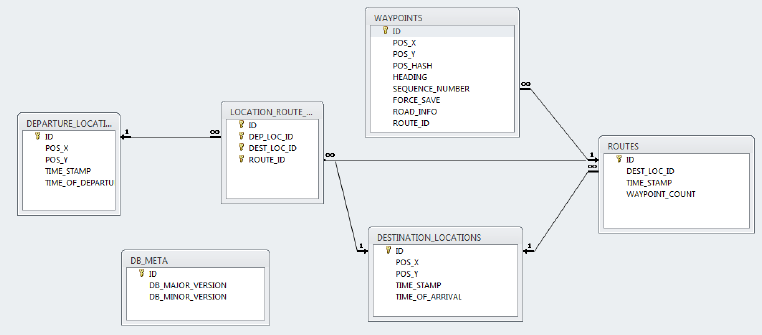
\includegraphics[width=0.9\textwidth]{Figures/baza_date.png}}
  \caption{Structura tabelelor de date și relațiile dintre ele}
\end{figure}

Tabelele din figura de mai sus sunt folosite pentru realiza structura întregii baze de date.
\vspace{6pt}
\\Tabela meta este folosită la identificarea versiunii bazei de date. Acest lucru este necesar pentru a detecta compatibilitatea și pentru a permite migrarea către o versiune mai recentă. 
\vspace{6pt}
\\Datele înregistrate sunt separate în puncte de plecare, destinații, rute și waypoint-uri. O rută este întotdeauna formată din mai multe waypoint-uri, unul sau mai multe puncte de plecare și una sau mai multe destinații. Ruta (waypoint-urile) sunt stocate numai o singură dată, în timp ce toate punctele de plecare și destinațiile sunt stocate. În acest fel, numărul de destinații poate influența probabilitatea rutei.
\vspace{6pt}
\\Accesul la date se face prin SQLite. Toate datele stocate pot fi atât citite cât și modificate.


